\chapter{Personalized Treatment Effects}
\label{ch-personalized}


This chapter
is based on the work of Pearl et al, as reported in
Refs.
\cite{pearl-tian-2000} and
\cite{personalized-pearl-2021}.

Recall from Chapter \ref{ch-pot-out}
on Potential Outcomes (PO) 
and beyond, that
the average treatment effect ($ATE$) 
is defined as
$ATE=E[\rvy_1-\rvy_0]$.
The conditional $ATE$ ($CATE$) is defined as
the conditional expected value
$C$ATE$=E_{|\rvz=z}[\rvy_1-\rvy_0]$.


{\bf
Personalized Treatment Effect (PTE)}
theory
as envisioned by Pearl
is the study 
of
bounds
for personal (i.e., conditional)
 treatment
effects such as $CATE$. The
bounds given by PTE theory
are
as tight as possible,
depending on 
the available data,
and on what bnet model 
assumptions
the user is willing to make.
We say bounds, because 
it is not always possible
to give a point estimate
for $CATE$ and other
PTEs.
If a point estimate for $CATE$
is achievable, we say $CATE$
is identifiable.

One 
very promising
field in 
which PTE theory
can be applied
is in {\bf Personalized Causal Medicine}.
For example, suppose we want to
 use $CATE$, 
where the conditioning is on the
sex of the patient,
to advice a female  patient
to take a cancer drug or not.

\section{Goal of PTE theory}
In the introduction
to this chapter,
we described 
briefly
the goal of PTE theory. 
In this section,
we will describe it
in more detail.

Let

{\bf Average Treatment Effect}


\beqa
ATE &=& E_\s[y^\s_1-y^\s_0]
\\
&=&
P(\rvy_1=1)-P(\rvy_0=1)
\eeqa

{\bf Average Causal Effect}

\beq
ACE= P(\rvy=1|\cald\rvx=1)-P(\rvy=1|\cald\rvx=0)
\eeq

Note that
\beq
ACE=\underbrace{P(\rvy=1|\cald\rvx=1)}_{P(\rvy_1=1)}
-\underbrace{P(\rvy=1|\cald\rvx=0)}_{P(\rvy_0=1)}
=ATE\eeq


{\bf Probability of Necessity and Sufficiency}
\beq
PNS = P(\rvy_0=0, \rvy_1=1)
\eeq

{\bf Amonotonicity Measure}
\beq
AMM = P(\rvy_0=1, \rvy_1=0)
\eeq

\begin{claim}
\beq
PSN=P(\rvy_1-\rvy_0=1)
\eeq
\beq
AMM=P(\rvy_1-\rvy_0=-1)
\eeq
\end{claim}
\proof

$\rvy_1-\rvy_0=1$ iff ($\rvy_1=1$ and
$\rvy_0=0$).

$\rvy_1-\rvy_0=-1$ iff ($\rvy_1=0$ and
$\rvy_0=1$).
\qed

\begin{figure}[h!]
\centering
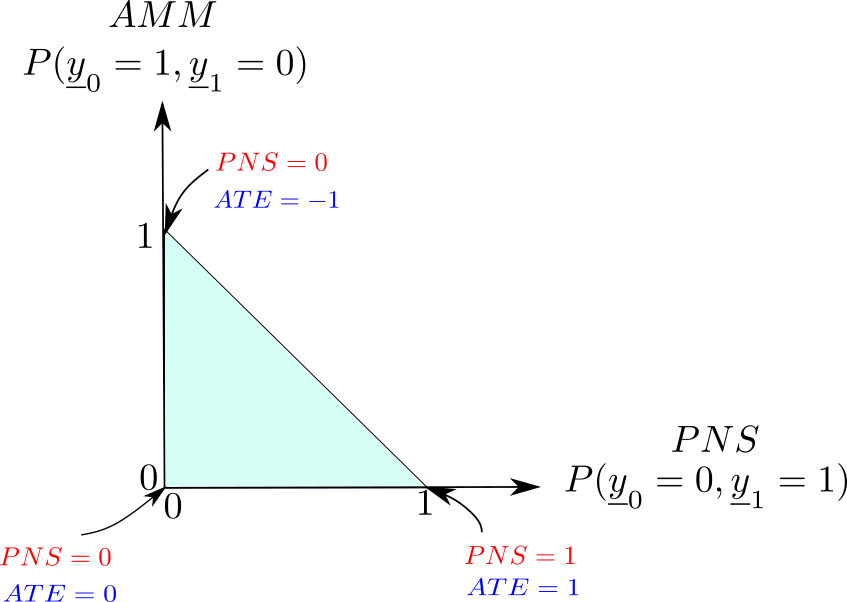
\includegraphics[width=3.5in]
{personalized/pns-ate.png}
\caption{Probability simplex 
with $x=P(\rvy_0=0, \rvy_1=1)$
and $y=P(\rvy_0=1, \rvy_1=0)$.
Values of $PNS$ and $ATE$
at corners
are given.
Points on line $x+y=1$ can only be
achieved if $P(1,1)=P(0,0)=0$. } 
\label{fig-pns-ate}
\end{figure}
\begin{claim}
\beq 
ATE = PNS - AMM
\eeq
\end{claim}
\proof
\beqa
ATE &=& E_\s[y^\s_1-y^\s_0]
\\
&=&E[\rvy_1-\rvy_0]
\\
&=&
\sum_{y}y[P(\rvy_1=y) -P(\rvy_0=y)]
\\
&=&
P(\rvy_1=1) -P(\rvy_0=1)
\\
&=&
\sum_{y_0}P(y_0, \rvy_1=1) - \sum_{y_1}P(\rvy_0=1, y_1)
\\
&=&
\underbrace{P(\rvy_0=0, \rvy_1=1)}_{PNS} -
\underbrace{P(\rvy_0=1, \rvy_1=0)}_{AMM}
\eeqa
\qed



See Fig.\ref{fig-pns-ate}
for a visualization
of the extreme values of
$PNS$ and the corresponding values
of $ATE$.


{\bf Conditional ATE (CATE)} is 
what we called $ATE_x$ in Chapter
\ref{ch-pot-out}

\beq
ATE_z = E_{\s|z}[\rvy_1^\s-\rvy_0^\s]
= \sum_\s P(\s|z)[\rvy_1^\s-\rvy_0^\s]
\eeq

\beq
ATE = \sum_z P(z) ATE_z
\eeq

{\bf Conditional ACE 
(CACE)} is what
is called
$ACE_z$ in Chapter \ref{ch-pot-out}.
Note that
$ACE_z=ATE_z$.

\begin{figure}[h!]
\centering
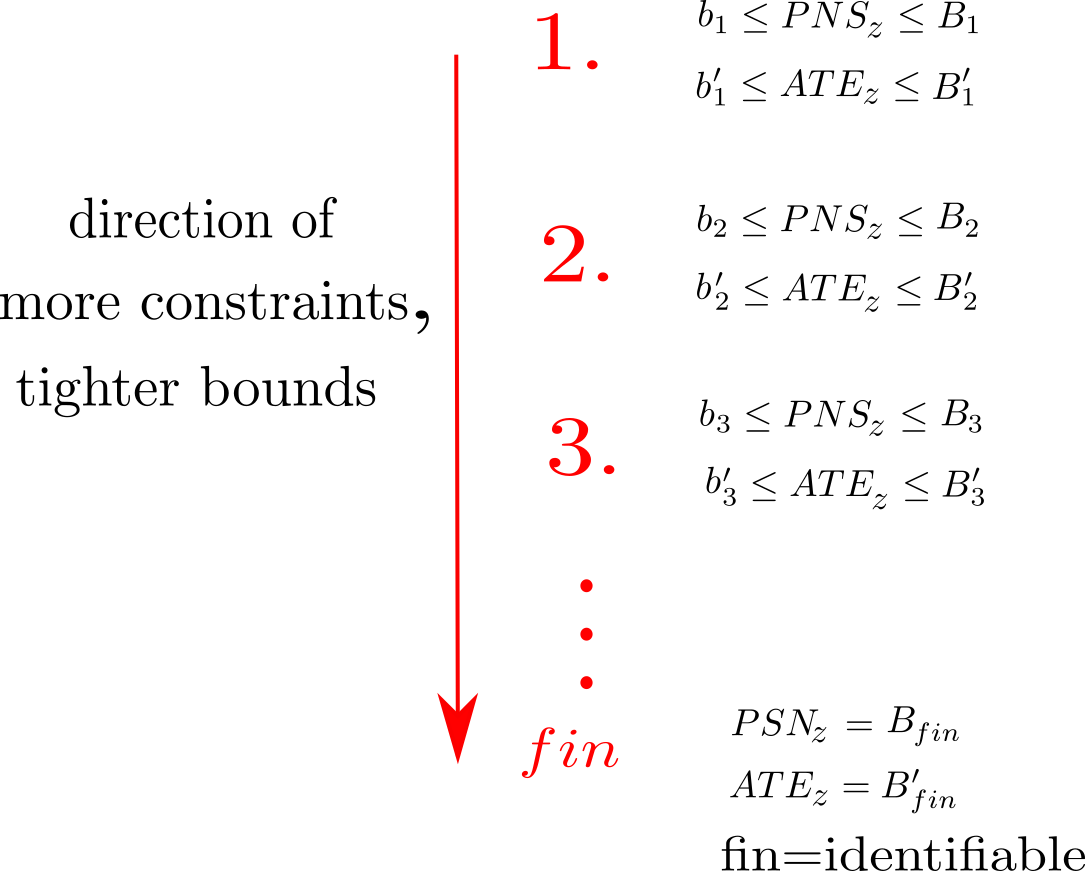
\includegraphics[width=3in]
{personalized/personalized-goal.png}
\caption{Increasingly
tighter observational bounds
$o_j, o'_j, O_j, O'_j$ 
for $PSN_z$ and $ATE_z$
ending in point bounds.
If a point bound is achievable
 for a quantity $Q$,
then we say $Q$
is identifiable.} 
\label{fig-personalized-goal}
\end{figure}

The goal of PTE theory, as
described by 
Fig.\ref{fig-personalized-goal}, is
to find
increasingly 
tighter bounds for
PTEs such as 
$PSN_z$ and $ATE_z$.


\section{Bnets for PTE theory}
\quad

Let $\ol{0}=1$ and $\ol{1}=0$.

Whenever we write $P(\rva=x, b)$, 
we mean $P(\rva=x, \rvb=b)$.

In this chapter, we will
not use the notation
$P(y)$ and $P(y')$
used by Pearl to
discuss PTE theory.
Instead, we will
use $P(\rvy=1)$ and
$P(\rvy=0)$
to denote his 
$P(y)$ and $P(y')$, respectively. 


On the other hand, 
in this chapter
we will change the names 
of variables $\rvd, \rvy, \rvz, \rvy(d)$
used 
in Chapter \ref{ch-pot-out} on Potential
Outcomes (PO)
to the names favored by Pearl.
Hence, we will replace
$\rvd, \rvy, \rvx, \rvy(d)$
by
$\rvx, \rvy, \rvz, \rvy_x$,
respectively.



PTE theory considers bnets of the form
Fig.\ref{fig-pte-bnet}.
The bnet considered in Rubin's
PO theory
is a very simple special case
of this where the box
labeled ``multiple nodes"
is absent and there is an
arrow pointing
from $\rvz$ to $\rvx$.


\begin{figure}[h!]
$$
\xymatrix{
&*++++[F]{\text{multiple nodes}}\ar@{<->}[ldd]
\ar@{<->}[r]
&*++[F-o]{\rvz}\ar[rd]\ar[d]
\\
&&\rvy_0\ar[d]
&\rvy_1\ar[ld]
\\
\rvx\ar[rr]
&&\rvy
}$$
\caption{Type of Bnet
considered in PTE theory.
The box labeled ``multiple nodes"
contains various observed 
and hidden nodes with
arrows
to or from node $\rvx$
and to or from
node $\rvz$.
$\rvz$ can be a multinode.
$\rvz$ 
is shown
as hidden but
could be observed instead.
}
\label{fig-pte-bnet}
\end{figure}

The TPM, printed in blue,
 for node $\rvy$
of bnet Fig.\ref{fig-pte-bnet}
is as follows:


\beq\color{blue}
P(y|y_0, y_1, x)=\delta(y, y_x)
\label{eq-tpm-y-yx}
\eeq

This TPM is used 
frequently
in PTE theory.  If $x$ is an argument
of $P()$, this TPM implies that one
can swap $\rvy=y_x$
and $\rvy_x=y_x$
inside $P()$. For example,
\beqa
P(y_0,y_1,x)
&=&
P({\color{red}\rvy_x}=y_x,
 y_{\ol{x}},x)
\\
&=&
P({\color{red}\rvy}=y_x,
 y_{\ol{x}},x)
\eeqa

According to Pearl, the defining
property of $y_x$ is that 


\beq
P(\rvy_x=y)=P(\rvy=y|\cald\rvx=x)
\eeq
This is also a
consequence of bnet Fig.\ref{fig-pte-bnet}
and the TPM Eq.(\ref{eq-tpm-y-yx}).
Indeed, 
$\cald\rvx=x$
means one should amputate
all arrows entering
node $\rvx$, and one should set
the TMP of $\rvx$ to a delta
function centered at $x$.
If that is done, then
the value
of $\rvy$ and $\rvy_x$ must
be equal, 
because of the TPM at node $\rvy$
is a delta function
enforcing this equality.


\section{Probabilities Relevant to PTE theory}
\beq
P^{x', y'}_{x,y}=
P(\rvy_{x'}=y'|x,y)
\eeq

{\bf observational (non-causal)
 probabilities}
\beq
O_{x,y}= P(\rvx=x,\rvy=y)
\eeq

\beq
O_{y|x}= P(\rvy=y|\rvx=x)
\eeq

\beq
\pi_x = P(\rvx=x)
\eeq

{\bf experimental (causal)
 probabilities}

\beq
E_{y|x}= P(\rvy_x=y)
\eeq
Note that 
\beqa
ATE&=&
P(\rvy_1=1)-P(\rvy_0=1)
\\
&=&
E_{1|1}-E_{1|0}
\\
&=& E_{1|1}+E_{0|0}-1
\eeqa


\newcommand{\PN}[0]{PN^{0,0}_{1,1}}
\newcommand{\PS}[0]{PS^{1,1}_{0,0}}
{\bf Probability of Necessity ($\PN$)}
\beq
\PN = P^{0,0}_{1,1}
\eeq


{\bf Probability of Sufficiency ($\PS$)}
\beq
\PS=P^{1,1}_{0,0}
\eeq




{\bf Probability of 
Necessity and Sufficiency (PNS)}

\beq
PNS=
P(\rvy_0=0, \rvy_1=1)
\eeq

{\bf Amonotonicity Measure (AMM)}

\beq
AMM= 
P(\rvy_0=1, \rvy_1=0)
\eeq

{\bf Risk ratio or relative risk (RR)}
\beq
RR = \frac{O_{1|1}}
{O_{1|0}}
\eeq



{\bf Excess Risk Ratio (ERR)} 
\beq
ERR=
\frac{O_{1|1}-O_{1|0}}
{O_{1|1}}= 1 - \frac{1}{RR}
\eeq

{\bf Corrected ERR (CERR)}
\beq
CERR=
ERR +
\frac{O_{1|0}-E_{1|0}}{O_{1,1}}
\eeq


\begin{claim}\label{cl-p-y0-y1-x}


\beqa
P(y_0, y_1|x)
&=&
P(y_{\ol{x}}|x, \rvy=y_x)P(\rvy=y_x|x)
\\
&&\xymatrix{\\=}
\xymatrix{
&y_{\ol{x}}
\\
x\ar[ur]\ar[r]
&\rvy=y_x\ar[u]
}
\eeqa
\end{claim}
\proof

\beqa
P(y_0, y_1|x)
&=&
\frac{P(y_0, y_1, x)}{P(x)}
\\
&=&
\frac{P(y_{\ol{x}}, x, \rvy=y_x)}{P(x)}
\\
&=&
\frac{P(y_{\ol{x}}|x, \rvy=y_x)P(x, \rvy=y_x)}{P(x)}
\\
&=&
P(y_{\ol{x}}|x, \rvy=y_x)P(\rvy=y_x|x)
\eeqa
\qed 

\begin{claim}
\beq
\underbrace{PNS}_{
P(\rvy_0=0, \rvy_1=1)
}
=\PN
 O_{1,1} + 
\PS O_{0,0}
\eeq
Hence, if we know
any two of $(\PN, \PS, PNS)$,
we can calculate the 
third.
\end{claim}
\proof
\begin{align}
P(y_0,y_1)
&=
\sum_xP(y_0,y_1|x)P(x)
\\
&=
\sum_x P(y_{\ol{x}}|x, \rvy=y_x)P(x,\rvy=y_x)\quad
\text{(see Claim \ref{cl-p-y0-y1-x}.)}
\\&=
\left\{
\begin{array}{l}
\quad P(y_1|\rvx=0, \rvy=y_0)P(\rvx=0, \rvy=y_0)
\\
+ P(y_0|\rvx=1, \rvy=y_1)P(\rvx=1, \rvy=y_1)
\end{array}
\right.
\end{align}
Thus,

\begin{align}
P(\rvy_0=0, \rvy_1=1)
&=
\left\{
\begin{array}{l}
\quad P(\rvy_1=1|\rvx=0, \rvy=0)P(\rvx=0, \rvy=0)
\\
+ P(\rvy_0=0|\rvx=1, \rvy=1)P(\rvx=1, \rvy=1)
\end{array}
\right.
\\
&=
\PS O_{0,0}
+
\PN O_{1,1}
\end{align}
\qed

To 
translate
from 
our notation 
to the notation
used by Tian and Pearl in
Ref.\cite{pearl-tian-2000},
 replace $P(\rvy_1=i,
 \rvy_0=j, \rvx=k)\rarrow p_{i,j,k}$
$O_{1,0}\rarrow P(x,y') $,
$O_{0|1}\rarrow P(y'|x)$, 
$ E_{0|1}\rarrow P(y'_x)$, etc.


\section{Symmetry}


Define $\sim$ to 
be an operator that swaps zeros and ones 
in $P(\rvy_0=y, \rvy_1=y', x)$.
Hence

\beq
[P(\rvy_0=y, \rvy_1=y', \rvx=x)]^\sim=
P(\rvy_1=\ol{y}, \rvy_0=\ol{y'}, \rvx=\ol{x})
\eeq

\beq 
(P^{x',y'}_{x,y})^\sim= P^{\ol{x'}, \ol{y'}}_{\ol{x}, \ol{y}}
\eeq

\beq
(O_{x,y})^\sim = O_{\ol{x},\ol{y}}
\eeq

\beq
(O_{y|x})^\sim = O_{\ol{y}|\ol{x}}
\eeq


\beq
(\pi_x)^\sim =\pi_{\ol{x}}
\eeq


\beq
(\PN)^\sim=\PS,\quad (\PS)^\sim=\PN
\eeq

\beq
(PNS)^\sim= PNS
\eeq

\beq
(RR)^\sim=
\frac{O_{0|0}}{O_{0|1}}
\eeq

Recall 

\beq
ERR=\frac{O_{1|1}-O_{1|0}}{O_{1|1}}=1-\frac{1}{RR}
\eeq
Therefore, define

\beq
(ERR)^\sim=
\frac{O_{0|0}-O_{0|1}}
{O_{0|0}}
=1 - \frac{1}{(RR)^\sim}
\eeq

Note that

\beqa
O_{1|1}-O_{1|0}&=&
O_{1|1}+O_{0|0}-1
\\&=&
O_{0|0}-O_{0|1}
\\&=&
(O_{1|1}-O_{1|0})^\sim
\eeqa


\section{Linear Programming Problem}

{\bf Probability Simplex}

\beq
\cals=\left\{P(y_0,y_1, x):
\begin{array}{l}
P(y_0,y_1, x)\geq 0
\\
y_0, y_1, x\in\bool
\\
\sum_{y_0=0}^1
\sum_{y_1=0}^1
\sum_{x=0}^1
P(y_0,y_1, x)
=1
\end{array}
\right\}\eeq

Note that $\cals$ has 7 degrees of freedom (dofs).


\begin{enumerate}

\item
{\bf experimental (causal) constraints 
  on $\cals$} 
{\color{red}(2 constraints)}\footnote{
$E_{0|x}$ follows from
$E_{0|x}=1-E_{1|x}$.}

\beq
E_{1|x}=P(\rvy_x=1)=\sum_{x'}
\sum_{y'}
P(\rvy_x=1, \rvy_{\ol{x}}=y', \rvx=x') \quad \text{for $x\in\bool$}
\eeq

\item
{\bf observational (non-causal)
 constraints on $\cals$} 
{\color{red}(3 constraints)}

\beq
O_{x, y}=P(x,y)=
\sum_{y'}
P(\rvy_x=y, \rvy_{\ol{x}}=y', x)
\quad\text{for $(x,y)\in\{(0,1),(1,0),(1,1)\}$}
\eeq
\end{enumerate}

$\cals$ has 7 dofs but the 
3 observational constraints
reduce the number of dofs to 4.
The 5 observational 
and experimental constraints
 reduce the number of dofs
to 2.
$\cals$ is embedded in $\RR^8$
and then the 6 constraints (unit
probability, 2 observational
and 3 experimental)
reduce it
 to the interior
of a  6 or less sided figure
 in $\RR^2$. 

Henceforth, we will
refer to the observational
 and experimental 
constraints together
as the {\bf minimal 
constraints}.

\beqa
PNS &=&
P(\rvy_0=0,\rvy_1=1)
\\
&=&
\sum_x P(\rvy_0=0,\rvy_1=1, x)
\eeqa

\beqa
\PN
&=&
 P(\rvy_0=0|\rvx=1,\rvy=1)
\\
&=&
\frac{P(\rvy_0=0, \rvy_1=1, \rvx=1)
}{O_{1,1}}
\eeqa

\beqa
\PS
&=&
 P(\rvy_1=1|\rvx=0,\rvy=0)
\\
&=&
\frac{P(\rvy_0=0, \rvy_1=1, \rvx=0)
}{O_{0,0}}
\eeqa



\section{Special constraints}
\begin{itemize}
\item
{\bf Exogeneity (a.k.a., no-confounding)}
holds for simplex $\cals$
if
$\rvy_x\perp \rvx$ for $x\in\bool$.
 Hence

\beq
\underbrace{P(\rvy_x=1)}_{E_{1|x}}
=P(\rvy_x=1|x)=
\underbrace{P(\rvy=1|x)}_{O_{1|x}}
\quad \text{for $x\in \bool$}
\eeq
Exogeneity gives {\color{red}2 constraints}.

Note that exogeneity
is the same thing as identifiability 
of $P(\rvy_x=y)=P(\rvy=y|\cald\rvx=x)$.
But identifiability
(i.e., do-identifiability) is a more 
general concept. One can speak
of the identifiability of $P(y_x|z)$
or of $P(y_0, y_1, a)$, etc.
In general,
any expression with 
do operators is do-identifiable
if it can be expressed 
as an expression without 
do-operators.

\item
{\bf Strong Exogeneity} holds 
for simplex $\cals$
if $(\rvy_0, \rvy_1)_{joint}
\perp \rvx$. Hence

\beq
P(y_0,y_1|x)=P(y_0, y_1)
\label{eq-strong-exogen}
\eeq
Strong exogeneity gives {\color{red} 3 constraints}.
Strong exogeneity implies
exogeneity
but not the converse.\footnote{In
this book, we use both 
$(\rva, \rvb)_\&\perp \rvx$
and $(\rva, \rvb)_{joint}\perp \rvx$.
When we write $(\rva, \rvb)_\&\perp \rvx$,
we mean that
$\rva\perp \rvx$
and $\rvb\perp\rvx$,
or, equivalently,
$P(a|x)=P(a)$
and $P(b|x)=P(b)$.
When we write
$(\rva, \rvb)_{joint}\perp \rvx$
or simply $(\rva, \rvb)\perp \rvx$,
we mean $P(a,b|x)=P(a,b)$.
Summing
$P(a,b|x)=P(a,b)$
over $a$ gives
$P(b|x)=P(b)$,
and summing it
over $b$ gives 
$P(a|x)=P(a)$.
Hence we see that
 $(\rva, \rvb)_{joint}\perp \rvx$
implies
$(\rva, \rvb)_\&\perp \rvx$
but not the converse.
If $\rva$ and $\rvb$ are independent at
fixed $\rvx$ so that 
$P(a,b|x)=P(a|x)P(b|x)$ then
$(\rva, \rvb)_{joint}\perp \rvx$
iff
$(\rva, \rvb)_\&\perp \rvx$
}
\item
{\bf Monotonicity}\footnote{
This property is called monotonicity
 because
it's equivalent to the statement
that $y_0^\s\leq y_1^\s$ for 
all individuals $\s$
in the population.
Indeed, $y_0^\s\leq y_1^\s$
includes the 3 cases $(y_0^\s, y_1^\s)=
(0,0), (1, 1), (0,1)$, but
excludes the only other
case, namely $(1,0)$.}
 holds for simplex $\cals$ if $AMM=P(\rvy_0=1,
 \rvy_1=0)=0$. Equivalently,

\beq
\sum_x P(\rvy_0=1, \rvy_1=0, x)=0
\eeq
which is true iff

\beq
 P(\rvy_0=1, \rvy_1=0, x)=0\quad
\text{for $x\in\bool$}
\eeq
Monotonicity gives {\color{red} 2 
constraints}.

Note that when $AMM=0$, $PSN=ATE$.
\end{itemize}



\begin{claim}
Monotonicity and exogeneity 
together imply strong exogeneity.
\end{claim}
\proof
Let $a\in \bool$.
\beqa
P(\rvy_a=\ol{a}, x)&=&
\sum_{a'}P(\rvy_a=\ol{a}, \rvy_{\ol{a}}=a', x)
\\
&=&P(\rvy_a=\ol{a}, \rvy_{\ol{a}}=\ol{a}, x)
\quad\text{(by monotonicity)}
\eeqa
Thus,

\beq 
P(\rvy_a=\ol{a}|\rvx=a)=P(\rvy_a=\ol{a},
 \rvy_{\ol{a}}=\ol{a}|\rvx=a)
\label{eq-pm-with-cond}
\eeq
and
\beq 
P(\rvy_a=\ol{a})=P(\rvy_a=\ol{a},
 \rvy_{\ol{a}}=\ol{a})
\label{eq-pm-without-cond}
\eeq
By exogeneity, 
the left hand side of Eq.(\ref{eq-pm-with-cond})
and the left hand side of Eq.(\ref{eq-pm-without-cond})
are equal,
so the right hand sides 
of those equations must be equal too.

\beq
P(\rvy_a=\ol{a},
 \rvy_{\ol{a}}=\ol{a}|\rvx=a)=
P(\rvy_a=\ol{a},
 \rvy_{\ol{a}}=\ol{a})
\eeq
This immediately implies\footnote{
If $x\in \bool$
and $P(a,\rvx=0)=P(a)P(\rvx=0)$,
then $P(a)- P(a,\rvx=0)=
P(a)[1-P(\rvx=0)]$,
so $ P(a,\rvx=1)= P(a)P(\rvx=1)$}

\beq
P(\rvy_a=\ol{a},
 \rvy_{\ol{a}}=\ol{a}|x)=
P(\rvy_a=\ol{a},
 \rvy_{\ol{a}}=\ol{a})
\eeq
for $x\in \bool$.
This gives for $a=0$
\beq
P(\rvy_0=1,
 \rvy_{1}=1|x)=
P(\rvy_0=1,
 \rvy_{1}=1)
\eeq
and for $a=1$
\beq
\underbrace{P(\rvy_1=0,
 \rvy_{0}=0|x)}_{
P(
 \rvy_{0}=0, \rvy_1=0|x)
}
=
\underbrace{
P(\rvy_1=0,
 \rvy_{0}=0)}_{P9
 \rvy_{0}=0,\rvy_1=0)}
\eeq
Monotonicity itself gives

\beq
 P(\rvy_0=1, \rvy_1=0|x)=0=
P(\rvy_0=1, \rvy_1=0)
\eeq
The remaining strong exogeneity constraint, given by
\beq
 P(\rvy_0=0, \rvy_1=1|x)=P(\rvy_0=0, \rvy_1=1)
\;,
\eeq
follows because 
\beq
\sum_{y_0,y_1}P(y_0, y_1|x)=
\sum_{y_0,y_1}P(y_0, y_1)=1
\eeq


\qed

\section{Matrix representation of probabilities}

Suppose $\eps_x(y_0, y_1)$
for $x,y_0,y_1\in \bool$
 are eight vectors 
in a vector space $V$.
$\eps_x(y_0, y_1)$ will only be used 
at position $(y_0,y_1)$
of a $2\times 2$ matrix,
where the positions are
 defined as follows:

\beq
\xymatrix@R=.7pc@C=.7pc{
y_1
\\
1\ar[u]
&(0,1)
&(1,1)
\\
0\ar@{-}[u]
&(0,0)
&(1,0)
\\
\ar@{-}[u]
\ar@{-}[r]
&0\ar@{-}[r]
&1\ar[r]
&y_0
}
\eeq
When $\eps_x(y_0, y_1)$
is used inside a $2\times 2$ 
matrix, we will not write
the argument $(y_0, y_1)$,
leaving it implicit, unless
confusion may arise.
Thus, for example, we will
represent $\Pmat{\eps_0(0,1)}{0}{0}{0}$
by $\Pmat{\eps_0}{0}{0}{0}$.



For $x\in \bool$, let
\begin{subequations}
\beq
P_{\rvy_0, \rvy_1, \rvx}(0,0,x)=
\Pmat{0}{0}{\eps_x}{0}
\eeq

\beq
P_{\rvy_0, \rvy_1, \rvx}(0,1,x)=
\Pmat{\eps_x}{0}{0}{0}
\eeq

\beq
P_{\rvy_0, \rvy_1, \rvx}(1,0,x)=
\Pmat{0}{0}{0}{\eps_x}
\eeq


\beq
P_{\rvy_0, \rvy_1, \rvx}(1,1,x)=
\Pmat{0}{\eps_x}{0}{0}
\eeq
\label{eq-prob-mats}
\end{subequations}


Define a map
$\calp[\quad]:V\rarrow \RR$
that we will call the
{\bf matrix representation 
of probabilities (MRP)} (mnemonic, Mr. P).
We will
assume that the map $\calp[\quad]$ is linear.
Hence, for instance,

\beq
\Pmat{4\eps_0+3\eps_1}
{-5\eps_0}
{0}
{0}=
4\Pmat{\eps_0}
{0}
{0}
{0}
+
3\Pmat{\eps_1}
{0}
{0}
{0}
-5
\Pmat{0}
{\eps_0}
{0}
{0}
\eeq
Note that

\beq
\Pmat{\eps_0+\eps_1}
{\eps_0+\eps_1}
{\eps_0+\eps_1}
{\eps_0+\eps_1}=1
\eeq


\beq 
E_{0|0}
=\Pmat{\eps_0+\eps_1}{0}{\eps_0+\eps_1}{0}
,\quad
O_{0,0}
=\Pmat{\eps_0}{0}{\eps_0}{0}
\eeq

\beq 
E_{0|1}
=\Pmat{0}{0}{\eps_0+\eps_1}{\eps_0+\eps_1}
,\quad
O_{1,0}
=\Pmat{0}{0}{\eps_1}{\eps_1}
\eeq

\beq 
E_{1|0}=\Pmat{0}{\eps_0+\eps_1}{0}{\eps_0+\eps_1}
,\quad
O_{0,1}=\Pmat{0}{\eps_0}{0}{\eps_0}
\eeq

\beq 
E_{1|1}=\Pmat{\eps_0+\eps_1}{\eps_0+\eps_1}{0}{0}
,\quad
O_{1,1}=\Pmat{\eps_1}{\eps_1}{0}{0}
\eeq

\beq
\PN O_{1,1}=\Pmat{\eps_1}{0}{0}{0}
\eeq

\beq
\PS O_{0,0}=\Pmat{\eps_0}{0}{0}{0}
\eeq

\beq
PNS =\Pmat{\eps_0+\eps_1}{0}{0}{0}
\eeq

\beq
AMM =\Pmat{0}{0}{0}{\eps_0+\eps_1}
\eeq

\beq
ATE=PNS-AMM=
\Pmat{\eps_0+\eps_1}{0}{0}{-\eps_0-\eps_1}
\eeq

\beq 
P(\rvy=0)=O_{0,0}+O_{1,0}=
\Pmat{\eps_0}{0}{\eps_0+\eps_1}{\eps_1}
\eeq

\beq 
P(\rvy=1)=O_{0,1}+O_{1,1}=
\Pmat{\eps_1}{\eps_0+\eps_1}{0}{\eps_0}
\eeq
When $AMM=0$, 
\beq 
P(\rvy=1)|_{AMM=0}=
\Pmat{\eps_1}{\eps_0+\eps_1}{0}{0}
\eeq


\begin{claim}
In general,

\beq
O_{x,1}\leq E_{1|x} \leq 1-O_{x,0}
\quad\text{for $x\in \bool$}
\;.
\eeq
In other words,

\beq
O_{1,1}\leq E_{1|1} \leq 1-O_{1,0}
\eeq
\beq
O_{0,1}\leq E_{1|0} \leq 1-O_{0,0}
\eeq
With monotonicity, we get the tighter bounds

\beq
\overbrace{
O_{1,1} +
\underbrace{O_{0,1}}_{new}
}^{P(\rvy=1)}
\leq 
E_{1|1}\leq 1- O_{1,0}
\eeq
\beq
O_{0,1}\leq E_{1|0}
\leq 
\overbrace{
1- O_{0,0}-\underbrace{O_{1,0}}_{new}
}^{P(\rvy=1)}
\eeq

\end{claim}
\proof

\beq
O_{1,1}\leq E_{1|1} \leq 
\underbrace{1-O_{1,0}}
_{O_{1,1}+O_{0,0}+O_{0,1}}
\eeq
has the MRP


\beq
\Pmat{\eps_1}{\eps_1}{0}{0}
\leq
\Pmat{\eps_0+\eps_1}{\eps_0+\eps_1}{0}{0}
\leq
\Pmat{\eps_1}{\eps_1}{0}{0}
+
\Pmat{\eps_0}{0}{\eps_0}{0}
+
\Pmat{0}{\eps_0}{0}{\eps_0}
\eeq
which is obviously true.

\beq
O_{0,1}\leq E_{1|0} \leq 
\underbrace{1-O_{0,0}}
_{O_{1,1}+O_{0,1}+O_{1,0}}
\eeq
has the MRP

\beq
\Pmat{0}{\eps_0}{0}{\eps_0}
\leq
\Pmat{0}{\eps_0+\eps_1}{0}{\eps_0+\eps_1}
\leq
\Pmat{\eps_1}{\eps_1}{0}{0}
+
\Pmat{0}{\eps_0}{0}{\eps_0}
+
\Pmat{0}{0}{\eps_1}{\eps_1}
\eeq
which is obviously true.

\beq
P(\rvy=1)|_{AMM=0}\leq E_{1|1}
\eeq
has the MRP 

\beq
\Pmat{\eps_1}{\eps_0+\eps_1}{0}{0}
\leq
\Pmat{\eps_0+\eps_1}{\eps_0+\eps_1}{0}{0}
\eeq
which is obviously true.

\beq
E_{1|0}|_{AMM=0}\leq
P(\rvy=1)|_{AMM=0}
\eeq
has the MRP

\beq
\Pmat{0}{\eps_0+\eps_1}{0}{0}
\leq
\Pmat{\eps_1}{\eps_0+\eps_1}{0}{0}
\eeq
which is obviously true.
\qed



\section{Bounds for unspecified bnet}

\begin{claim}\label{cl-basic-bound-joint}
If $P(a,b)$ is a probability 
distribution, then
\beq
\max\{0, P(a) + P(b)-1\}\leq 
P(a,b)\leq \min\{P(a), P(b)\}
\eeq
\end{claim}
\proof
$P(a|b)\leq 1$ 
and $P(b|a)\leq 1$
implies $P(a,b)\leq P(b)$
and $P(a,b)\leq P(a)$.
Hence, $P(a,b)\leq \min\{P(a), P(b)\}$.

\begin{align}
P(a) + P(b) -1
&=
\sum_{a', b'} P(a',b')
\underbrace
{[\delta(a,a')+\delta(b,b')
-1]}_{T}
\\
&\leq
P(a,b)\quad 
\text{($T$ biggest
when $a=a'$ and $b=b'$)}
\end{align}
\qed


\begin{figure}[h!]
\centering

\includegraphics[width=3in]
{personalized/bounds-minimal.png}
\caption{Minimal bounds
for $PNS$.
$PNS$ is larger
than maximum of the purple segments
and smaller than the
minimum of the green ones.
The purple segment of almost zero
length represents zero.
The green segment 
interrupted by a thin green
line represents $O_{0,0} + O_{1,1}$.
Note that $\sum_x O_{x,0}+ 
\sum_x O_{x,1}=1$. When
monotonicity holds,
$PNS$ equals $E_{1,1}+E_{0,0}-1$
which is the purple
segment marked with a star.
} 
\label{fig-bounds-minimal}
\end{figure}

\begin{claim} Minimal bounds 
\label{cl-minimal-bounds}
(see Fig.\ref{fig-bounds-minimal})

If the minimal
constraints hold for simplex $\cals$, 
then

\beq
\max\left\{
\begin{array}{c}
0
\\
E_{1|1}+E_{0|0}-1
\\
E_{0|0}-\sum_x O_{x,0}
\\
E_{1|1}-\sum_x O_{x,1}
\end{array}
\right\}
\leq
PNS
\leq
\min\left\{
\begin{array}{c}
E_{1|1}
\\
E_{0|0}
\\
O_{1,1}+O_{0,0}
\\
E_{1|1}+E_{0|0}-O_{1,1}-O_{0,0}
\end{array}
\right\}
\eeq

\beq
\max\left\{
\begin{array}{c}
0
\\
\frac{E_{0|0}-\sum_x O_{x,0}}
{O_{1,1}}
\end{array}
\right\}
\leq
\PN
\leq
\min\left\{
\begin{array}{c}
1
\\
\frac{E_{0|0}-O_{0,0}}
{O_{1,1}}
\end{array}
\right\}
\eeq

\beq
\max\left\{
\begin{array}{c}
0
\\
\frac{E_{1|1}-\sum_x O_{x,1}}
{O_{0,0}}
\end{array}
\right\}
\leq
\PS
\leq
\min\left\{
\begin{array}{c}
1
\\
\frac{E_{1|1}-O_{1,1}}
{O_{0,0}}
\end{array}
\right\}
\eeq

Note that $\sum_x O_{x,y}=P(\rvy=y)$
for $y=0,1$. 

Let $A_0=E_{0|0}-\sum_x O_{x,0}$,
 $A_1=E_{1|1}-\sum_x O_{x,1}$,
and $A=E_{1|1}+E_{0|0}-1$.
Note that $A,A_0$ and $A_1$ are all lower bounds 
of $PNS$, and $A=A_0+A_1$, 
so we could remove $A_0$ and $A_1$
from the max\{\;\} argument. But that 
would mean that 
cases where we knew $E_{0|0}$
or $E_{1|1}$but not both, would be unaccounted for.
\end{claim}
\proof
These bounds 
were copied directly 
from Ref.\cite{pearl-tian-2000},
except the notation was changed.
Ref.\cite{pearl-tian-2000}
explains how Balke, 
in his 1995 Ph.D. thesis under Pearl, 
 derived these bounds 
using his software based on standard 
algorithms  
from Linear Programming.
In certain cases, we have slightly 
rewritten
the bounds
from Ref.\cite{pearl-tian-2000} to
 exhibit more explicitly their 
symmetry under swaps of zeros and ones.
For example,
instead of using
$(E_{1|0}, E_{1|1})$
as parameters,
we use $(E_{1|1}, E_{0|0})$.

These bounds can be easily 
proven using the MRP.

The first two lines of the
bound for $PNS$ are a simple
consequence of 
Claim \ref{cl-basic-bound-joint}.
Indeed, Claim \ref{cl-basic-bound-joint}
implies  
\beq
\max\left\{\begin{array}{l}
0\\
 P(y_0)+P(y_1)-1
\end{array}\right\}
\leq
P(y_0, y_1)
\leq
\min\left\{\begin{array}{l}
P(y_0)\\
 P(y_1)
\end{array}\right\}
\eeq
When $y_0=0, y_1=1$, we get
\beq
\max\left\{\begin{array}{l}
0\\
 E_{0|0}+E_{1|1}-1
\end{array}\right\}
\leq
PNS
\leq
\min\left\{\begin{array}{l}
 E_{0|0}\\
 E_{1|1}
\end{array}\right\}
\eeq
\qed



\begin{claim}\label{cl-personal-exogen}
If minimal
and exogeneity constraints hold
for simplex $\cals$, then


\beq
\max\left\{\begin{array}{l}
0\\
O_{1|1}+O_{0|0}-1
\end{array}\right\}
\leq
PNS
\leq
\min\left\{\begin{array}{l}
O_{1|1}\\
O_{0|0}
\end{array}\right\}
\eeq

\beq
\max\left\{\begin{array}{l}
0\\
ERR
\end{array}\right\}
\leq
\PN
\leq
\min\left\{\begin{array}{l}
1\\
\frac{O_{0|0}}{O_{1|1}}
\end{array}\right\}
\eeq

\beq
\max\left\{\begin{array}{l}
0\\
(ERR)^\sim
\end{array}\right\}
\leq 
\PS
\leq
\min\left\{\begin{array}{l}
1\\
\frac{O_{1|1}}{O_{0|0}}
\end{array}\right\}
\eeq

\end{claim}
\proof
Just
replace $E_{y|x}$ by $O_{y|x}$
in the minimal bounds given in
Claim \ref{cl-minimal-bounds}.
\qed








\begin{claim}
If the minimal and 
strong exogeneity constraints
 hold for simplex $\cals$,
then the inequalities 
for exogeneity Claim \ref{cl-personal-exogen}
hold.
In addition,
\beq
\PN =\frac{PNS}{O_{1|1}}
\eeq
and

\beq
\PS =\frac{PNS}{O_{0|0}}
\eeq
\end{claim}
\proof
\beqa
\PN O_{1|1}&=&
P(\rvy_0=0, \rvy=1|\rvx=1)
\\
&=&
P(\rvy_0=0, \rvy_1=1)
\\
&=&PNS
\eeqa

\beqa
\PS O_{0|0}&=&
P(\rvy_1=1, \rvy=0|\rvx=0)
\\
&=&
P(\rvy_0=0, \rvy_1=1)
\\
&=& PNS
\eeqa
\qed


\begin{claim}\label{cl-pm-mono}
If the minimal
and monotonicity constraints hold
 for simplex $\cals$, then




\beq
PNS=E_{1|1}+E_{0|0}-1
\eeq

\beq
\PN=\frac{E_{0|0}-\sum_x O_{x,0}}{O_{1,1}}
=
\frac{\sum_x O_{x,1}-E_{1|0}}{O_{1,1}}
=
CERR
\eeq

\beq
\PS = \frac{E_{1|1}-\sum_x O_{x,1}}{O_{0,0}}
= \frac{\sum_x O_{x,0}-E_{0|1}}{O_{0,0}}
= (CERR)^\sim
\eeq



\end{claim}
\proof
These results can be easily 
proven using the MRP.

Note that

\beqa
\frac{\sum_x O_{x,1}-E_{1|0}}{O_{1,1}}
&=& 
\frac{ O_{1|1}\pi_1 + O_{1|0}(1-\pi_1)
-E_{1|0}}{O_{1|1}\pi_1}
\\
&=&
1-\frac{O_{1|0}}{O_{1|1}}
+\frac{O_{1|0}-E_{1|0}}{O_{1,1}}
\\
&=& CERR
\eeqa

\qed


\begin{claim}
If the minimal,
exogeneity and monotonicity 
constraints hold
 for simplex $\cals$, then
$PNS$, $\PN$,$\PS$ are identifiable,
and


\beq
PNS = O_{1|1}+O_{0|0}-1
\eeq

\beq
\PN
=\frac{O_{0|0}-\sum_x O_{x, 0}}{O_{1,1}}
=\frac{\sum_x O_{x, 1}-O_{1|0}}{O_{1,1}}
=ERR
\eeq

\beq
\PS=\frac{O_{1|1}-\sum_x O_{x,1}}{O_{0,0}}
=\frac{\sum_x O_{x,0}-O_{0|1}}{O_{0,0}}
=(ERR)^\sim
\eeq

\end{claim}
\proof
Set $E_{y|x}=O_{y|x}$ in Claim 
\ref{cl-pm-mono}.
\qed

\section{Bounds for specific bnet family}
Define
\beq
E_{*|*,z} = E_{0|0, z} + E_{1|1, z}=ATE_z+1
\eeq

\beq
O_{*,*|z} = O_{0,0|z} + O_{1,1| z}
\eeq
Recall the minimal bounds
\beq
\max\left\{
\begin{array}{c}
0
\\
E_{*|*}-1
\\
E_{0|0}-\sum_x O_{x,0}
\\
E_{1|1}-\sum_x O_{x,1}
\end{array}
\right\}
\leq
PNS
\leq
\min\left\{
\begin{array}{c}
E_{1|1}
\\
E_{0|0}
\\
O_{*,*}
\\
E_{*|*}-O_{*,*}
\end{array}
\right\}
\eeq

\begin{claim}\label{cl-pre-backdoor-bounds}
If $\rvz\cap de(\rvx)=\emptyset$, then
\beq
\sum_z P(z)
\max\left\{
\begin{array}{l}
0\\
E_{*|*,z}-1
\\
E_{0|0,z}-\sum_x O_{x,0|z}
\\
E_{1|1,z}-\sum_x O_{x,1|z}
\end{array}
\right\}
\leq
PNS
\leq
\sum_z P(z)
\min\left\{
\begin{array}{l}
E_{1|1,z}
\\
E_{0|0,z}
\\
O_{*,*|z}
\\
E_{*|*,z}-O_{*,*|z}
\end{array}
\right\}
\label{eq-pre-backdoor-bounds}
\eeq
\end{claim}
\proof
Same as minimal bounds,
except conditioned on $z$.
\qed

\begin{claim}
If $\rvz$ satisfies the backdoor adjustment
criterion relative $(\rvx,\rvy)$,
then

\beq
\sum_z P(z)
\max\left\{
\begin{array}{l}
0
\\
O_{*|*,z}
\end{array}
\right\}
\leq
PNS
\leq
\sum_z P(z)
\min
\left\{
\begin{array}{l}
O_{1|1,z}
\\
O_{0|0,z}
\end{array}
\right\}
\eeq
\end{claim}
\proof
Satisfaction 
of the backdoor criterion implies that
\beq
\underbrace{P(y|x,z)}_{O_{y|x,z}}
=\underbrace{P(y_x|z)}_{E_{y|x,z}}
\eeq
Replace $E_{y|x,z}$ by $O_{y|x,z}$
in Eq.(\ref{eq-pre-backdoor-bounds}).
\qed





We say $\rvz$
is a {\bf partial mediator}
relative to $(\rvx, \rvy)$ if
 $\rvy_x\perp(\rvx,
\rvz_{\ol{x}})|\rvz_x$ for $x\in \bool$.
See Fig.\ref{fig-partial-mediator}
for an example.

\begin{figure}[h!]
$$\xymatrix{
*++[F-o]{\rvu}\ar[d]\ar[r]
&\rvz\ar[rd]
\\
\rvx\ar[ru]
&&\rvy
}$$
\caption{Example of a bnet in  
which $\rvz$ is a partial mediator
relative to $(\rvx, \rvy)$.
}
\label{fig-partial-mediator}
\end{figure}

\begin{claim} (Bounds if $\rvz$ 
is partial 
mediator)

If $\rvz$ is a partial mediator
relative to $(\rvx, \rvy)$, then

\beq
\max\left\{
\begin{array}{c}
0
\\
E_{*|*}-1
\\
E_{0|0}-\sum_x O_{x,0}
\\
E_{1|1}-\sum_x O_{x,1}
\end{array}
\right\}
\leq
PNS
\leq
\min\left\{
\begin{array}{c}
E_{1|1}
\\
E_{0|0}
\\
O_{*,*}
\\
E_{*|*}-O_{*,*}
\\
new
\end{array}
\right\}
\eeq

\beq
new=
\sum_z\sum_{z'}\min
\left\{\begin{array}{l}
O_{1|1,z}\\O_{0|0,z'}
\end{array}\right\}
\min
\left\{\begin{array}{l}
P(z_1)
\\
P(z'_0)
\end{array}\right\}
\eeq
\end{claim}
\proof
\qed

\begin{claim} (Bounds if $\rvz$ 
is a pure mediator)

If  $\xymatrix{&\rvz\ar[rd]\\\rvx\ar[ru]&&\rvy}$, then


\beq
\max\left\{
\begin{array}{c}
0
\\
E_{*|*}-1
\\
E_{0|0}-\sum_x O_{x,0}
\\
E_{1|1}-\sum_x O_{x,1}
\end{array}
\right\}
\leq
PNS
\leq
\min\left\{
\begin{array}{c}
E_{1|1}
\\
E_{0|0}
\\
O_{*,*}
\\
E_{*|*}-O_{*,*}
\\
new
\end{array}
\right\}
\eeq

\beq
new=
\sum_z\sum_{z'}
\indi(z\neq z')
\min
\left\{\begin{array}{l}
\sum_x O_{x,1|z}\\
\sum_x O_{x,0|z'}
\end{array}\right\}
\min
\left\{\begin{array}{l}
P(z| \rvx=1)
\\
P(z'| \rvx=0)
\end{array}\right\}
\eeq
\end{claim}
\proof
\qed